These are general tips about few \LaTeX{} and \LyX{} functionalities.

\section{Copy and paste raw \protect\LaTeX{} code}

Sometimes it is necessary to insert raw \LaTeX{} code in your document,
\LyX{} has a dedicated environment for that (\textsf{Insert} \textsf{\lyxarrow}
\textsf{Tex code}). By using the paste command (\textsf{CTRL + V})
to copy text into that type of environment, you get as result that
everything is copied in a single line, all the carriage returns are
ignored. To paste exactly what you have copied, use the special paste
command which preserves the text formatting (\textsf{CTRL + SHIFT
+ V} or \textsf{Edit} \textsf{\lyxarrow{} Paste Special \lyxarrow Plain
Text}).

\section{Labels and cross-references\label{sec:label-and-cross}}

Labels are necessary to add cross-references in your thesis, use a
label for each element that you have to reference to (\textsf{Insert}
\textsf{\lyxarrow} \textsf{Label/Cross-reference}). These elements
are manly chapters, sections, subsections, figures, tables and algorithms.

This is Chapter \ref{chap:second-chapter}, Section \ref{sec:label-and-cross}.

\section{Figures}

Figures, but also tables and algorithms, must be placed inside a floating
environment. This type of \LaTeX{} environment is very useful and automagically
mix up text and images. Usually the \textsf{Here if possible} placement
option is good for all images (right click on \textsf{float: Figure}
then \textsf{Settings}). However, if the figure is not placed correctly
you may enable the \textsf{Ignore \LaTeX{} rules} option, usually that
option solves every problem.

Figure \ref{fig:image} shows an example of a very nice animal.

\begin{figure}[h]
\begin{centering}
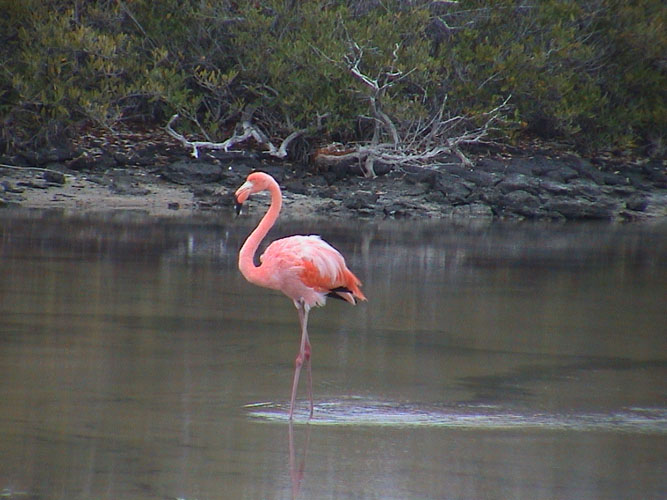
\includegraphics[width=0.5\columnwidth]{chapter-2/images/flamingo}
\par\end{centering}
\caption[Short caption of the figure]{\label{fig:image}Detailed caption of this marvelous animal}
\end{figure}
A rarely known feature of \LyX{} is the possibility to add the short
caption. The short caption is the description of the figure used in
the \textsf{List of Figures} section. Sometimes captions can be very
long, in this case it is better to use a shorter one that is more
readable in the page that lists all the figures. To add this caption,
right click on the description of figure, then \textsf{Insert short
title}.

It is not mandatory to add the short caption, it is only useful with
very long captions to ensure a better legibility of the \textsf{List
of Figures} section.

\subsection{Subfigures}

A very cool feature of \LaTeX 's figures is the possibility to have
subfigures. For example, if there are two figures that represent the
result of a test executed with two different values of a parameter,
then a subfigure is a good way to organize the images.

Figure \ref{fig:subfig-fauna} is an example of these subfigures.
References can be added to either the whole figure (Figure \ref{fig:subfig-fauna})
or each subfigure (Figure \ref{fig:fauna-squirrel} and Figure \ref{fig:fauna-peacock}).

\begin{figure}[h]
\hfill{}\subfloat[\label{fig:fauna-squirrel}A nice squirrel]{\centering{}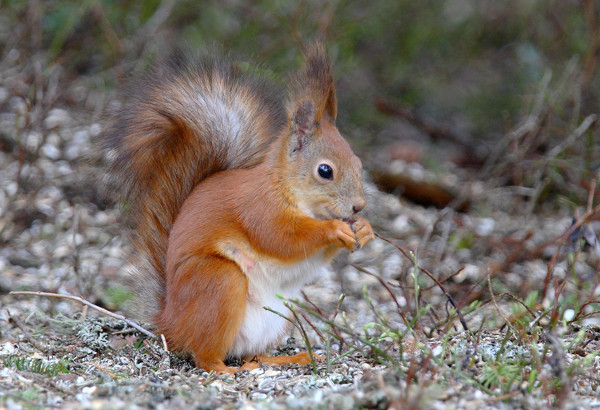
\includegraphics[width=0.45\columnwidth]{chapter-2/images/squirrel}}\hfill{}\subfloat[\label{fig:fauna-peacock}A beautiful peacock]{\centering{}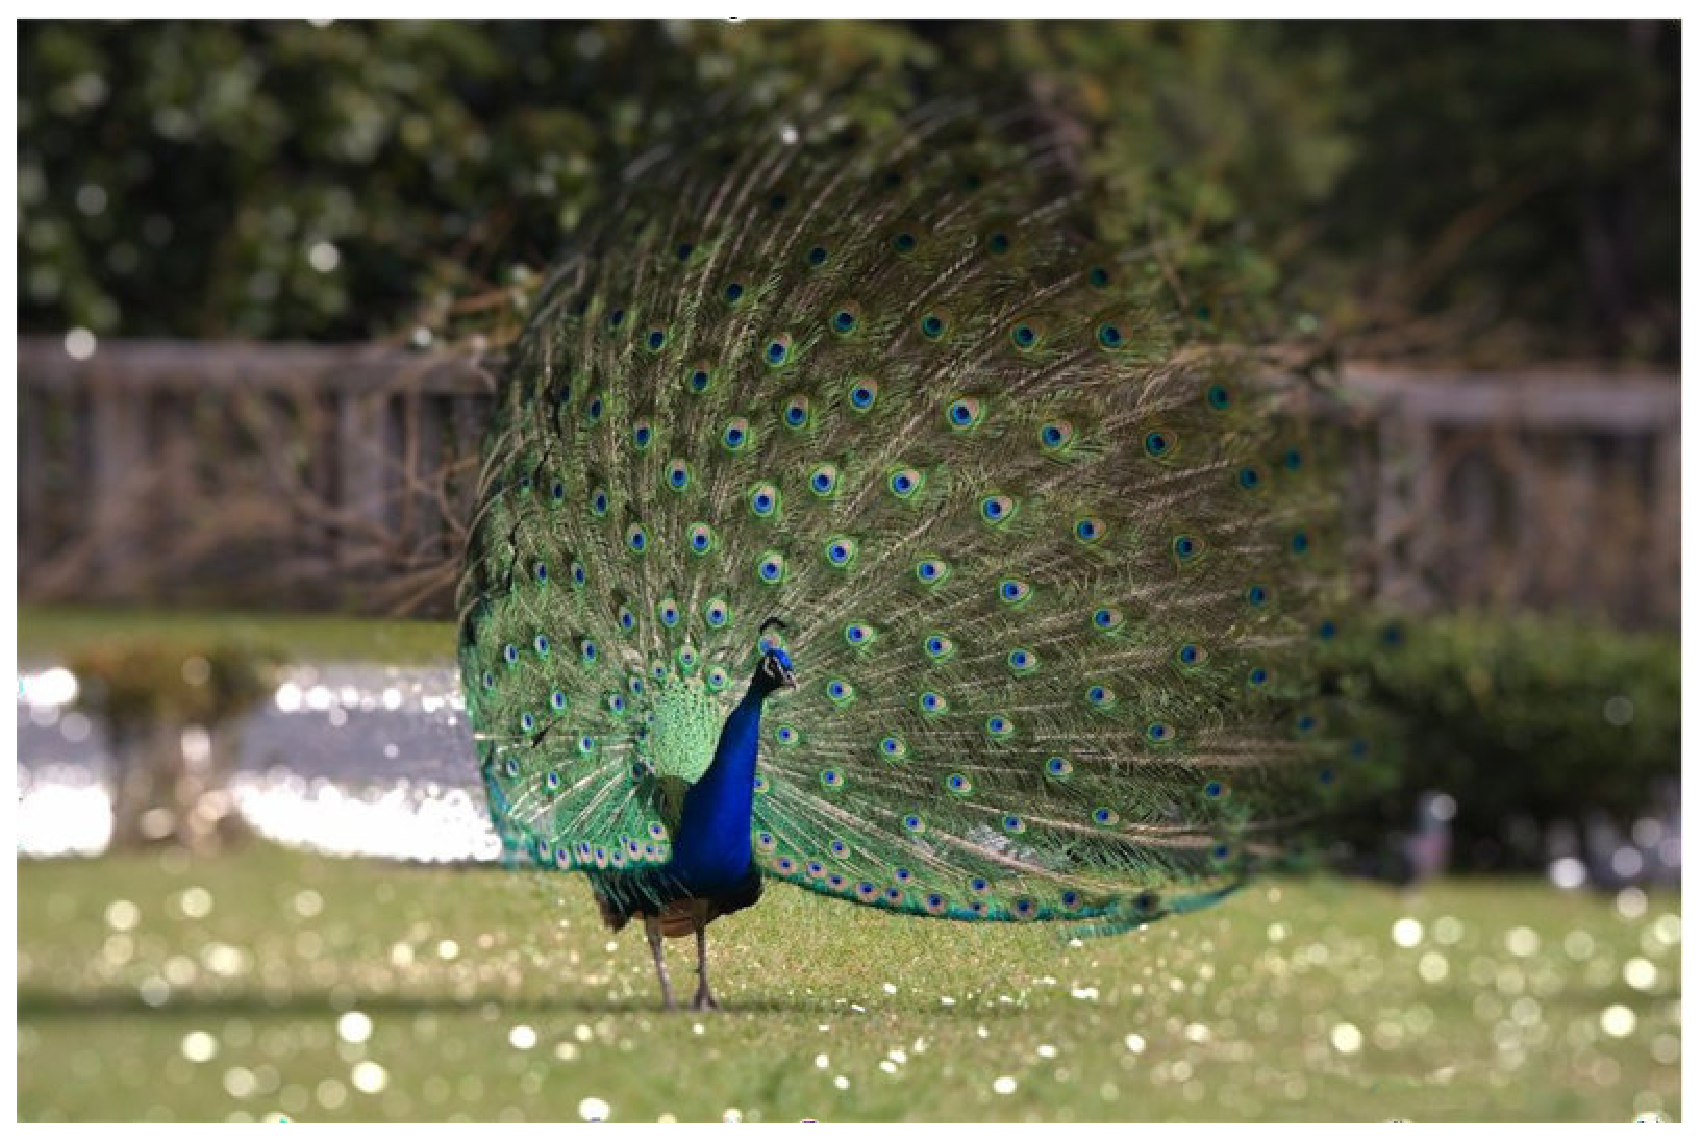
\includegraphics[width=0.45\columnwidth]{chapter-2/images/peacock}}\hfill{}

\caption{\label{fig:subfig-fauna}Fauna}

\end{figure}

\section{Tables}

The caption of tables must be placed before the table itself and not
after. As for figures, tables can have a short caption that is used
in the \textsf{List of Tables} section.

Academic publications, but also thesis, often use the so-called <<formal
table>>, an example of these particular style is showed in Table
\ref{tab:formal-table}

\begin{table}[h]
\centering{}\caption[Short caption of the table]{\label{tab:formal-table}Detailed caption of this beautiful table}
{\small{}}%
\begin{tabular}{ccccc}
\toprule 
 & \multicolumn{2}{c}{\textbf{Category}} &  & \tabularnewline
\cmidrule{2-3} 
 & \textbf{first} & \textbf{second} & \textbf{Number} & \textbf{Complexity}\tabularnewline
\midrule 
\textbf{Item A} & $\alpha$ & $\beta$ & $4$ & $\Omega\left(n\right)$\tabularnewline
\textbf{Item B} & $\gamma$ & $\delta$ & $2$ & $\Omega\left(n^{2}\right)$\tabularnewline
\bottomrule
\end{tabular}
\end{table}
To set this particular style, right click in a cell of the table then
\textsf{More} \textsf{\lyxarrow} \textsf{Settings} \textsf{\lyxarrow}
\textsf{Border}, here you can select the formal style.

\subsection{Wide tables}

Sometimes tables are too wide for the column's width of the page.
Rather than changing the table's content you can shrink it to fit
the available space. The font size will be smaller but this is, in
general, a good method to fix too wide tables such as Table \ref{tab:wide-table},
the result is showed in Table \ref{tab:wide-table-shrunk}.

\begin{table}[h]
\caption{\label{tab:wide-table}This table is very wide}

\centering{}%
\begin{tabular}{ccccc}
\toprule 
\textbf{Method} & \textbf{Parameter one} & \textbf{Parameter two} & \textbf{Parameter three} & \textbf{Parameter four}\tabularnewline
\midrule 
A & $1$ & $2$ & $3$ & $4$\tabularnewline
B & $5$ & $7$ & $9$ & $11$\tabularnewline
\bottomrule
\end{tabular}
\end{table}
\begin{table}[h]
\caption{\label{tab:wide-table-shrunk}This table is shrunk to fit the column's
width}

\centering{}\resizebox{\linewidth}{!}{%
\begin{tabular}{ccccc}
\toprule 
\textbf{Method} & \textbf{Parameter one} & \textbf{Parameter two} & \textbf{Parameter three} & \textbf{Parameter four}\tabularnewline
\midrule 
A & $1$ & $2$ & $3$ & $4$\tabularnewline
B & $5$ & $7$ & $9$ & $11$\tabularnewline
\bottomrule
\end{tabular}}
\end{table}
Another solution is to set the width of table's columns. To set it,
right click in a cell of the table then \textsf{More} \textsf{\lyxarrow}
\textsf{Settings} \textsf{\lyxarrow} \textsf{Table settings}, here
you can set the width.

\subsection{Space between rows}

Another common problem with tables is when rows of the table are too
close together, this problem is very frequent when rows contain mathematical
expressions such as Table \ref{tab:math-table}. With a simple command
it is possible to increase the space between rows as showed in Table
\ref{tab:math-table-big-rows}.

\begin{table}[h]
\caption{\label{tab:math-table}This table is a bit tight}

\centering{}%
\begin{tabular}{cc}
\toprule 
\textbf{Name} & \textbf{Formula}\tabularnewline
\midrule 
Gaussian integral & $\int_{0}^{+\infty}e^{-\frac{x^{2}}{2}}\text{dx}=\frac{1}{2}\sqrt{\frac{\pi}{2}}$\tabularnewline
Taylor series & $\sum_{n=0}^{\infty}\frac{f^{\left(n\right)}\left(a\right)}{n!}\left(x-a\right)^{n}$\tabularnewline
\bottomrule
\end{tabular}
\end{table}
\begin{table}[h]
\caption{\label{tab:math-table-big-rows}Math cheatsheet}

\centering{}\renewcommand*{\arraystretch}{1.5}%
\begin{tabular}{cc}
\toprule 
\textbf{Name} & \textbf{Formula}\tabularnewline
\midrule 
Gaussian integral & $ $$\int_{0}^{+\infty}e^{-\frac{x^{2}}{2}}\text{dx}=\frac{1}{2}\sqrt{\frac{\pi}{2}}$\tabularnewline
Taylor series & $\sum_{n=0}^{\infty}\frac{f^{\left(n\right)}\left(a\right)}{n!}\left(x-a\right)^{n}$\tabularnewline
\bottomrule
\end{tabular}
\end{table}

\section{Algorithms}

If you have to add some algorithms there is a dedicated \LyX{} environment.
As for tables, the caption of an algorithm must be placed before the
pseudo code of the algorithm, short captions can be used also for
algorithm. This placement of the caption may sound strange but is
justified by the fact that algorithms, but also tables, are read from
the top down, so the description must be placed before the content.
On the other side, figures are viewed like a painting, so the description
must be placed below the content.

\begin{algorithm}[h]
\begin{enumerate}
\item \caption[Short caption of the algorithm]{\label{alg:the-algorithm}Detailed caption of this complicated algorithm}
Wake up

\begin{enumerate}
\item drink a coffee
\item brush your teeth
\end{enumerate}
\item Go to work
\item Come back home
\item Go to sleep
\end{enumerate}
\end{algorithm}
Unfortunately \LyX{} does not support algorithm commands offered by
some \LaTeX{} packages (\texttt{\textbackslash If}, \texttt{\textbackslash While},
\ldots ) out of the box. It is possible to use custom modules to handle
those commands or use the 2.1 beta version that supports some of them
but, as for now, it is better to write directly \LaTeX{} code. This
template uses the \textsf{algorithmicx} package, refer to the manual
of that package (\url{http://www.ctan.org/pkg/algorithmicx}) for
the documentation of all the commands. Algorithm \ref{alg:best-algorithm-ever}
shows an example of the usage of some commands of the \textsf{algorithmicx}
package.

\begin{algorithm}[h]
\caption{\label{alg:best-algorithm-ever}Best algorithm ever}
\begin{algorithmic}[1]
	\State $s \gets \texttt{ALIVE}$ \Comment{Day of birth}
	\While{$ s \neq \texttt{EOL}$}
		\Repeat \Comment{Early morning, possibly}
			\State Try to wake up
		\Until{$s = \texttt{SLEEP}$}
		\State Drink a coffe \Comment{Even more than one}
		\State Brush your teeth
		\State Go to work \Comment{With a smile on your face}
		\State Come back home
		\State Go to sleep
	\EndWhile
\end{algorithmic}
\end{algorithm}

\section{Source code}

You may need to add some pieces of source code that you have written.
\LyX{} uses \textsf{listings} package to provide a customized environment
to insert source code (\textsf{Insert} \textsf{\lyxarrow{} Program
Listing}). Listings can have a caption, but \LyX{} does not add it
by default, if you want you can insert it (place the cursor inside
the listing environment, then \textsf{Insert \lyxarrow{} Caption}).

By default, the result that you get is pretty ugly as you can see
in the Listing \ref{lis:ugly-code}.

\begin{lstlisting}[caption={Program that computes your degree mark},label={lis:ugly-code}]
#include <stdlib.h>
#include <stdio.h>

/**
 * Main program
 */
int main(int argc, char *argv[])
{
	long double degree_mark = 0x42 * 042 * 0b00101010 * 0.001167;

	printf("Congratulations for your degree\n");
	printf("Your mark is %-3.0LfL\n", degree_mark);

	return EXIT_SUCCESS;
}
\end{lstlisting}

You need to set a couple of options (right click inside the source
code environment, then \textsf{Settings}) to get a good looking result.
The most important options are
\begin{description}
\item [{Font~style}] use a fixed-length font (\textsf{Font Family: Typewriter}),
it is useful to set a \textsf{Small} font size to compact large pieces
of source code. Breaking long lines is very important as well as hiding
nasty spaces (check \textsf{Break long lines} option, uncheck \textsf{Space
as symbol} and \textsf{Space in strings as symbol} options, set \textsf{Tabular
size} to $4$)
\item [{Line~numbering}] having the line numbering active is useful if
you have to refer to a particular statement when you are describing
you code
\item [{Language}] setting the proper language is important to have the
correct syntax highlighting
\end{description}
The Listing \ref{lis:beautiful-code} has the same code as the Listing
\ref{lis:ugly-code} but it has all the options mentioned before adjusted,
the result is way better that the other.

\begin{lstlisting}[caption={Program that computes your degree mark},label={lis:beautiful-code},basicstyle={\small\ttfamily},breaklines=true,commentstyle={\color{purple!60!black}},extendedchars=true,identifierstyle={\color{blue!50!black}},keywordstyle={\bfseries\color{green!50!black}},language=C,numbers=left,numberstyle={\footnotesize},showstringspaces=false,stringstyle={\color{orange!40!black}},tabsize=4,xleftmargin=2em]
#include <stdlib.h>
#include <stdio.h>

/**
 * Main program
 */
int main(int argc, char *argv[])
{
	long double degree_mark = 0x42 * 042 * 0b00101010 * 0.001167;

	printf("Congratulations for your degree\n");
	printf("Your mark is %-3.0LfL\n", degree_mark);

	return EXIT_SUCCESS;
}
\end{lstlisting}

If you have to insert more than one piece of code it can be useful
to copy the previously created environment and then modify it. This
saves you from setting the options every time you insert a new listing.

\section{URLs}

\LyX{} has a dedicated command to insert URLs (\textsf{Insert \lyxarrow{}
URL}) that must be used to insert each URL. The environment automatically
uses a typewrite font for the text, inserts a hyperlink to the URL
and, most importantly, breaks long URLs in multiple lines.

This is a URL added as simple text, http://this.is.not.the.correct.way.to.add.urls.in.lyx.documents.html.

This is a URL created with the \textsf{url} command, \url{http://this.is.the.correct.way.to.add.urls.in.lyx.documents.html}.

The \textsf{url} environment can be manually used, for example, in
the bibliography where URLs are not handled in a dedicated way. The
Listing \ref{lis:urls-bibliography} shows how to use the url command
in the bibliography.

\begin{lstlisting}[caption={How to insert URLs in the bibliography},label={lis:urls-bibliography},basicstyle={\small\ttfamily},breaklines=true,commentstyle={\color{purple!60!black}},extendedchars=true,identifierstyle={\color{blue!50!black}},keywordstyle={\bfseries\color{green!50!black}},language=TeX,numbers=left,numberstyle={\footnotesize},showstringspaces=false,stringstyle={\color{orange!40!black}},tabsize=4,xleftmargin=2em]
% this URL will not be broken into multiple lines and
% will NOT have a hyperlink
@article{
    ...
    howpublished = {http://google.com}
}

% this URL WILL be broken into multiple lines and
% WILL have a hyperlink
@article{
    ...
    howpublished = {\url{http://google.com}}
}
\end{lstlisting}


\section{\protect\LyX 's guides}

\LyX{} has a series of guides that describe all its features, if want
to exploit all the available functionalities you need to read them.
Those manuals are available directly in \LyX{} (for example, \textsf{Help}
\textsf{\lyxarrow{} Embedded Objects}).
